\documentclass[11pt,addpoints,answers]{exam}

%-----------------------------------------------------------------------------
% PACKAGES AND OTHER DOCUMENT CONFIGURATIONS
%-----------------------------------------------------------------------------

\usepackage[margin=1in]{geometry}
\usepackage{amsmath, amsfonts}
\usepackage{enumerate}
\usepackage{graphicx}
\usepackage{titling}
\usepackage{url}
\usepackage{xfrac}
\usepackage{natbib}
\usepackage{amssymb}
\usepackage{amsthm}
\usepackage{paralist}
\usepackage{epstopdf}
\usepackage{tabularx}
\usepackage{longtable}
\usepackage{multirow}
\usepackage{multicol}
\usepackage[colorlinks=true,urlcolor=blue]{hyperref}
\usepackage{algorithm}
\usepackage{algorithmicx}
\usepackage[noend]{algpseudocode}
\usepackage{float}
\usepackage{enumerate}
\usepackage{array}
\usepackage{environ}
\usepackage{times}
\usepackage{textcomp}
\usepackage{caption}
\usepackage{parskip} % For NIPS style paragraphs.
\usepackage[compact]{titlesec} % Less whitespace around titles
\usepackage[inline]{enumitem} % For inline enumerate* and itemize*
\usepackage{datetime}
\usepackage{comment}
% \usepackage{minted}
\usepackage{lastpage}
\usepackage{color}
\usepackage{xcolor}
\usepackage[final]{listings}
\usepackage{tikz}
\usetikzlibrary{shapes,decorations}
\usepackage{framed}
\usepackage{booktabs}
\usepackage{cprotect}
\usepackage{verbatimbox}
\usepackage{multicol}
\usepackage{hyperref}
\usepackage{subcaption}
\usepackage{mathtools} % For drcases
\usepackage{cancel}
\usepackage[many]{tcolorbox}
\usepackage{soul}
\usepackage[bottom]{footmisc}
\usepackage{bm}
\usepackage{wasysym}

\usepackage{tikz}
\usetikzlibrary{shapes.geometric}
\usetikzlibrary{positioning, arrows, automata}

\newtcolorbox[]{your_solution}[1][]{%
    % breakable,
    enhanced,
    nobeforeafter,
    colback=white,
    title=Your Answer,
    sidebyside align=top,
    box align=top,
    #1
}

%%%%%%%%%%%%%%%%%%%%%%%%%%%%%%%%%%%%%%%%%%%
% Rotated Column Headers                  %
%%%%%%%%%%%%%%%%%%%%%%%%%%%%%%%%%%%%%%%%%%%
\usepackage{adjustbox}
\usepackage{array}

%https://tex.stackexchange.com/questions/32683/rotated-column-titles-in-tabular

\newcolumntype{R}[2]{%
    >{\adjustbox{angle=#1,lap=\width-(#2)}\bgroup}%
    l%
    <{\egroup}%
}
\newcommand*\rot{\multicolumn{1}{R{45}{1em}}}% no optional argument here, please!


%%%%%%%%%%%%%%%%%%%%%%%%%%%%%%%%%%%%%%%%%%%
% Better numbering                        %
%%%%%%%%%%%%%%%%%%%%%%%%%%%%%%%%%%%%%%%%%%%

% \numberwithin{equation}{section} % Number equations within sections (i.e. 1.1, 1.2, 2.1, 2.2 instead of 1, 2, 3, 4)
% \numberwithin{figure}{section} % Number figures within sections (i.e. 1.1, 1.2, 2.1, 2.2 instead of 1, 2, 3, 4)
% \numberwithin{table}{section} % Number tables within sections (i.e. 1.1, 1.2, 2.1, 2.2 instead of 1, 2, 3, 4)

%%%%%%%%%%%%%%%%%%%%%%%%%%%%%%%%%%%%%%%%%%
% Custom commands                        %
%%%%%%%%%%%%%%%%%%%%%%%%%%%%%%%%%%%%%%%%%%

\newcommand{\vc}[1]{\boldsymbol{#1}}
\newcommand{\adj}[1]{\frac{d J}{d #1}}
\newcommand{\chain}[2]{\adj{#2} = \adj{#1}\frac{d #1}{d #2}}

\newcommand{\R}{\mathbb{R}}
\newcommand{\blackcircle}{\tikz\draw[black,fill=black] (0,0) circle (1ex);}
\renewcommand{\circle}{\tikz\draw[black] (0,0) circle (1ex);}

\newcommand{\emptysquare}{{\LARGE $\square$}\ \ }
\newcommand{\filledsquare}{{\LARGE $\boxtimes$}\ \ }
\newcommand{\emptycircle}{{\LARGE $\fullmoon$}\ \ }
\newcommand{\filledcircle}{{\LARGE $\newmoon$}\ \ }


% mathcal
\newcommand{\Ac}{\mathcal{A}}
\newcommand{\Bc}{\mathcal{B}}
\newcommand{\Cc}{\mathcal{C}}
\newcommand{\Dc}{\mathcal{D}}
\newcommand{\Ec}{\mathcal{E}}
\newcommand{\Fc}{\mathcal{F}}
\newcommand{\Gc}{\mathcal{G}}
\newcommand{\Hc}{\mathcal{H}}
\newcommand{\Ic}{\mathcal{I}}
\newcommand{\Jc}{\mathcal{J}}
\newcommand{\Kc}{\mathcal{K}}
\newcommand{\Lc}{\mathcal{L}}
\newcommand{\Mc}{\mathcal{M}}
\newcommand{\Nc}{\mathcal{N}}
\newcommand{\Oc}{\mathcal{O}}
\newcommand{\Pc}{\mathcal{P}}
\newcommand{\Qc}{\mathcal{Q}}
\newcommand{\Rc}{\mathcal{R}}
\newcommand{\Sc}{\mathcal{S}}
\newcommand{\Tc}{\mathcal{T}}
\newcommand{\Uc}{\mathcal{U}}
\newcommand{\Vc}{\mathcal{V}}
\newcommand{\Wc}{\mathcal{W}}
\newcommand{\Xc}{\mathcal{X}}
\newcommand{\Yc}{\mathcal{Y}}
\newcommand{\Zc}{\mathcal{Z}}

% mathbb
\newcommand{\Ab}{\mathbb{A}}
\newcommand{\Bb}{\mathbb{B}}
\newcommand{\Cb}{\mathbb{C}}
\newcommand{\Db}{\mathbb{D}}
\newcommand{\Eb}{\mathbb{E}}
\newcommand{\Fb}{\mathbb{F}}
\newcommand{\Gb}{\mathbb{G}}
\newcommand{\Hb}{\mathbb{H}}
\newcommand{\Ib}{\mathbb{I}}
\newcommand{\Jb}{\mathbb{J}}
\newcommand{\Kb}{\mathbb{K}}
\newcommand{\Lb}{\mathbb{L}}
\newcommand{\Mb}{\mathbb{M}}
\newcommand{\Nb}{\mathbb{N}}
\newcommand{\Ob}{\mathbb{O}}
\newcommand{\Pb}{\mathbb{P}}
\newcommand{\Qb}{\mathbb{Q}}
\newcommand{\Rb}{\mathbb{R}}
\newcommand{\Sb}{\mathbb{S}}
\newcommand{\Tb}{\mathbb{T}}
\newcommand{\Ub}{\mathbb{U}}
\newcommand{\Vb}{\mathbb{V}}
\newcommand{\Wb}{\mathbb{W}}
\newcommand{\Xb}{\mathbb{X}}
\newcommand{\Yb}{\mathbb{Y}}
\newcommand{\Zb}{\mathbb{Z}}

% mathbf lowercase
\newcommand{\av}{\mathbf{a}}
\newcommand{\bv}{\mathbf{b}}
\newcommand{\cv}{\mathbf{c}}
\newcommand{\dv}{\mathbf{d}}
\newcommand{\ev}{\mathbf{e}}
\newcommand{\fv}{\mathbf{f}}
\newcommand{\gv}{\mathbf{g}}
\newcommand{\hv}{\mathbf{h}}
\newcommand{\iv}{\mathbf{i}}
\newcommand{\jv}{\mathbf{j}}
\newcommand{\kv}{\mathbf{k}}
\newcommand{\lv}{\mathbf{l}}
\newcommand{\mv}{\mathbf{m}}
\newcommand{\nv}{\mathbf{n}}
\newcommand{\ov}{\mathbf{o}}
\newcommand{\pv}{\mathbf{p}}
\newcommand{\qv}{\mathbf{q}}
\newcommand{\rv}{\mathbf{r}}
\newcommand{\sv}{\mathbf{s}}
\newcommand{\tv}{\mathbf{t}}
\newcommand{\uv}{\mathbf{u}}
\newcommand{\vv}{\mathbf{v}}
\newcommand{\wv}{\mathbf{w}}
\newcommand{\xv}{\mathbf{x}}
\newcommand{\yv}{\mathbf{y}}
\newcommand{\zv}{\mathbf{z}}

% mathbf uppercase
\newcommand{\Av}{\mathbf{A}}
\newcommand{\Bv}{\mathbf{B}}
\newcommand{\Cv}{\mathbf{C}}
\newcommand{\Dv}{\mathbf{D}}
\newcommand{\Ev}{\mathbf{E}}
\newcommand{\Fv}{\mathbf{F}}
\newcommand{\Gv}{\mathbf{G}}
\newcommand{\Hv}{\mathbf{H}}
\newcommand{\Iv}{\mathbf{I}}
\newcommand{\Jv}{\mathbf{J}}
\newcommand{\Kv}{\mathbf{K}}
\newcommand{\Lv}{\mathbf{L}}
\newcommand{\Mv}{\mathbf{M}}
\newcommand{\Nv}{\mathbf{N}}
\newcommand{\Ov}{\mathbf{O}}
\newcommand{\Pv}{\mathbf{P}}
\newcommand{\Qv}{\mathbf{Q}}
\newcommand{\Rv}{\mathbf{R}}
\newcommand{\Sv}{\mathbf{S}}
\newcommand{\Tv}{\mathbf{T}}
\newcommand{\Uv}{\mathbf{U}}
\newcommand{\Vv}{\mathbf{V}}
\newcommand{\Wv}{\mathbf{W}}
\newcommand{\Xv}{\mathbf{X}}
\newcommand{\Yv}{\mathbf{Y}}
\newcommand{\Zv}{\mathbf{Z}}

% bold greek lowercase
\newcommand{\alphav     }{\boldsymbol \alpha     }
\newcommand{\betav      }{\boldsymbol \beta      }
\newcommand{\gammav     }{\boldsymbol \gamma     }
\newcommand{\deltav     }{\boldsymbol \delta     }
\newcommand{\epsilonv   }{\boldsymbol \epsilon   }
\newcommand{\varepsilonv}{\boldsymbol \varepsilon}
\newcommand{\zetav      }{\boldsymbol \zeta      }
\newcommand{\etav       }{\boldsymbol \eta       }
\newcommand{\thetav     }{\boldsymbol \theta     }
\newcommand{\varthetav  }{\boldsymbol \vartheta  }
\newcommand{\iotav      }{\boldsymbol \iota      }
\newcommand{\kappav     }{\boldsymbol \kappa     }
\newcommand{\varkappav  }{\boldsymbol \varkappa  }
\newcommand{\lambdav    }{\boldsymbol \lambda    }
\newcommand{\muv        }{\boldsymbol \mu        }
\newcommand{\nuv        }{\boldsymbol \nu        }
\newcommand{\xiv        }{\boldsymbol \xi        }
\newcommand{\omicronv   }{\boldsymbol \omicron   }
\newcommand{\piv        }{\boldsymbol \pi        }
\newcommand{\varpiv     }{\boldsymbol \varpi     }
\newcommand{\rhov       }{\boldsymbol \rho       }
\newcommand{\varrhov    }{\boldsymbol \varrho    }
\newcommand{\sigmav     }{\boldsymbol \sigma     }
\newcommand{\varsigmav  }{\boldsymbol \varsigma  }
\newcommand{\tauv       }{\boldsymbol \tau       }
\newcommand{\upsilonv   }{\boldsymbol \upsilon   }
\newcommand{\phiv       }{\boldsymbol \phi       }
\newcommand{\varphiv    }{\boldsymbol \varphi    }
\newcommand{\chiv       }{\boldsymbol \chi       }
\newcommand{\psiv       }{\boldsymbol \psi       }
\newcommand{\omegav     }{\boldsymbol \omega     }

% bold greek uppercase
\newcommand{\Gammav     }{\boldsymbol \Gamma     }
\newcommand{\Deltav     }{\boldsymbol \Delta     }
\newcommand{\Thetav     }{\boldsymbol \Theta     }
\newcommand{\Lambdav    }{\boldsymbol \Lambda    }
\newcommand{\Xiv        }{\boldsymbol \Xi        }
\newcommand{\Piv        }{\boldsymbol \Pi        }
\newcommand{\Sigmav     }{\boldsymbol \Sigma     }
\newcommand{\Upsilonv   }{\boldsymbol \Upsilon   }
\newcommand{\Phiv       }{\boldsymbol \Phi       }
\newcommand{\Psiv       }{\boldsymbol \Psi       }
\newcommand{\Omegav     }{\boldsymbol \Omega     }

%%%%%%%%%%%%%%%%%%%%%%%%%%%%%%%%%%%%%%%%%%%
% Code highlighting with listings         %
%%%%%%%%%%%%%%%%%%%%%%%%%%%%%%%%%%%%%%%%%%%

\definecolor{bluekeywords}{rgb}{0.13,0.13,1}
\definecolor{greencomments}{rgb}{0,0.5,0}
\definecolor{redstrings}{rgb}{0.9,0,0}
\definecolor{light-gray}{gray}{0.95}

\newcommand{\MYhref}[3][blue]{\href{#2}{\color{#1}{#3}}}%

\definecolor{dkgreen}{rgb}{0,0.6,0}
\definecolor{gray}{rgb}{0.5,0.5,0.5}
\definecolor{mauve}{rgb}{0.58,0,0.82}

\lstdefinelanguage{Shell}{
  keywords={tar, cd, make},
  %keywordstyle=\color{bluekeywords}\bfseries,
  alsoletter={+},
  ndkeywords={python, py, javac, java, gcc, c, g++, cpp, .txt, octave, m, .tar},
  %ndkeywordstyle=\color{bluekeywords}\bfseries,
  identifierstyle=\color{black},
  sensitive=false,
  comment=[l]{//},
  morecomment=[s]{/*}{*/},
  commentstyle=\color{purple}\ttfamily,
  %stringstyle=\color{red}\ttfamily,
  morestring=[b]',
  morestring=[b]",
  backgroundcolor = \color{light-gray}
}

\lstset{columns=fixed, basicstyle=\ttfamily,
    backgroundcolor=\color{light-gray},xleftmargin=0.5cm,frame=tlbr,framesep=4pt,framerule=0pt}


%%%%%%%%%%%%%%%%%%%%%%%%%%%%%%%%%%%%%%%%%%%
% Custom box for highlights               %
%%%%%%%%%%%%%%%%%%%%%%%%%%%%%%%%%%%%%%%%%%%

% Define box and box title style
\tikzstyle{mybox} = [fill=blue!10, very thick,
    rectangle, rounded corners, inner sep=1em, inner ysep=1em]

% \newcommand{\notebox}[1]{
% \begin{tikzpicture}
% \node [mybox] (box){%
%     \begin{minipage}{\textwidth}
%     #1
%     \end{minipage}
% };
% \end{tikzpicture}%
% }

\NewEnviron{notebox}{

\begin{tikzpicture}
\node [mybox] (box){
    \begin{minipage}{\textwidth}
        \BODY
    \end{minipage}
};
\end{tikzpicture}
}

%%%%%%%%%%%%%%%%%%%%%%%%%%%%%%%%%%%%%%%%%%%
% Commands showing / hiding solutions     %
%%%%%%%%%%%%%%%%%%%%%%%%%%%%%%%%%%%%%%%%%%%

%% To HIDE SOLUTIONS (to post at the website for students), set this value to 0: 
\def\issoln{0}
% \def\issoln{1}
% Some commands to allow solutions to be embedded in the assignment file.
\ifcsname issoln\endcsname \else \def\issoln{1} \fi
% Default to an empty solutions environ.
\NewEnviron{soln}{}{}
\if\issoln 1
% Otherwise, include solutions as below.
\RenewEnviron{soln}{
    \leavevmode\color{red}\ignorespaces
    % \textbf{Solution} \BODY
    \BODY
}{}
\fi

%% To HIDE TAGS set this value to 0:
\def\showtags{0}
%%%%%%%%%%%%%%%%
\ifcsname showtags\endcsname \else \def\showtags{1} \fi
% Default to an empty tags environ.
\NewEnviron{tags}{}{}
\if\showtags 1
% Otherwise, include solutions as below.
\RenewEnviron{tags}{
    \fbox{
    \leavevmode\color{blue}\ignorespaces
    \textbf{TAGS:} \texttt{\url{\BODY}}
    }
    \vspace{-.5em}
}{}
\fi

%%%%%%%%%%%%%%%%%%%%%%%%%%%%%%%%%%%%%%%%%%%
% Commands for customizing the assignment %
%%%%%%%%%%%%%%%%%%%%%%%%%%%%%%%%%%%%%%%%%%%

\newcommand{\courseName}{10-301/10-601 Introduction to Machine Learning (Fall 2021)}
\newcommand{\hwName}{Homework 4: Logistic Regression}
\newcommand{\dueDate}{Monday, October 11, 2021 11:59 PM}


\title{\textsc{\hwName}
%\thanks{Compiled on \today{} at \currenttime{}}
} % Title


\author{\courseName\\
\url{http://mlcourse.org} \\
OUT: Saturday, October 2, 2021 \\
DUE: \dueDate{} \\ 
TAs: Gopi Krishna, Roshan, Justin, Youngjoo, Jingyun
}

\date{}

%%%%%%%%%%%%%%%%%%%%%%%%%%%%%%%%%%%%%%%%%%%%%%%%%
% Useful commands for typesetting the questions %
%%%%%%%%%%%%%%%%%%%%%%%%%%%%%%%%%%%%%%%%%%%%%%%%%

\newcommand \expect {\mathbb{E}}
\newcommand \mle [1]{{\hat #1}^{\rm MLE}}
\newcommand \map [1]{{\hat #1}^{\rm MAP}}
\newcommand \argmax {\operatorname*{argmax}}
\newcommand \argmin {\operatorname*{argmin}}
\newcommand \code [1]{{\tt #1}}
\newcommand \datacount [1]{\#\{#1\}}
\newcommand \ind [1]{\mathbb{I}\{#1\}}

%%%%%%%%%%%%%%%%%%%%%%%%%%
% Document configuration %
%%%%%%%%%%%%%%%%%%%%%%%%%%

% Don't display a date in the title and remove the white space
\predate{}
\postdate{}
\date{}

% Don't display an author and remove the white space
%\preauthor{}
%\postauthor{}

%%%%%%%%%%%%%%%%%%
% Begin Document %
%%%%%%%%%%%%%%%%%% 

\begin{document}

\maketitle



\begin{notebox}
\paragraph{Summary} In this assignment, you will build a sentiment polarity analyzer, which will be capable of analyzing the overall sentiment polarity (positive or negative) . In the Written component, you will warm up by deriving stochastic gradient descent updates for logistic regression. Then in the Programming component, you will implement a logistic regression model as the core of your natural language processing system.
\end{notebox}
\section*{START HERE: Instructions}
\begin{itemize}

\item \textbf{Collaboration Policy}: Please read the collaboration policy here: \url{http://www.cs.cmu.edu/~mgormley/courses/10601/syllabus.html}

\item\textbf{Late Submission Policy:} See the late submission policy here: \url{http://www.cs.cmu.edu/~mgormley/courses/10601/syllabus.html}

\item\textbf{Submitting your work:} You will use Gradescope to submit
  answers to all questions and code. Please
  follow instructions at the end of this PDF to correctly submit all your code to Gradescope.

  \begin{itemize}
    
 % COMMENT IF NOT USING CANVAS
\begin{comment}
  \item \textbf{Canvas:} Canvas (\url{https://canvas.cmu.edu}) will be
    used for quiz-style problems (e.g. multiple choice, true / false,
    numerical answers). Grading is done automatically.
    %
    You may only \textbf{submit once} on canvas, so be sure of your
    answers before you submit. However, canvas allows you to work on
    your answers and then close out of the page and it will save your
    progress.  You will not be granted additional submissions, so
    please be confident of your solutions when you are submitting your
    assignment.
    %
    {\color{red} The above is true for future assignments, but this one
    allows {\bf unlimited submissions}.}
\end{comment}
    
  % COMMENT IF NOT USING GRADESCOPE
   \item \textbf{Written:} For written problems such as short answer, multiple choice, derivations, proofs, or plots, please use the provided template. Submissions can be handwritten onto the template, but should be labeled and clearly legible. If your writing is not legible, you will not be awarded marks. Alternatively, submissions can be written in LaTeX. 
   Each derivation/proof should be completed in the boxes provided. If you do not follow the template, your assignment may not be graded correctly by our AI assisted grader.

  %   COMMENT IF NOT USING GRADESCOPE AUTOGRADER
  \item \textbf{Programming:} You will submit your code for programming questions on the homework to Gradescope (\url{https://gradescope.com}). After uploading your code, our grading scripts will autograde your assignment by running your program on a virtual machine (VM). When you are developing, check that the version number of the programming language environment (e.g. Python 3.9.6, OpenJDK 11.0.11, g++ 7.5.0) and versions of permitted libraries (e.g.  \texttt{numpy} 1.21.2 and \texttt{scipy} 1.7.1) match those used on Gradescope. You have 10 Gradescope programming submissions. We recommend debugging your implementation on your local machine (or the Linux servers) and making sure your code is running correctly first before submitting you code to Gradescope.

  \end{itemize}
  
\item\textbf{Materials:} The data that you will need in order to complete this assignment is posted along with the writeup and template on Piazza.

\end{itemize}


\begin{notebox}
\paragraph{Linear Algebra Libraries} When implementing machine learning algorithms, it is often convenient to have a linear algebra library at your disposal. In this assignment, Java users may use EJML\footnote{\url{https://ejml.org}} or ND4J\footnote{\url{https://javadoc.io/doc/org.nd4j/nd4j-api/latest/index.html}} and C++ users may use Eigen\footnote{\url{http://eigen.tuxfamily.org/}}. Details below. 
%
(As usual, Python users have NumPy.)
%
\begin{description}
\item[EJML for Java] EJML is a pure Java linear algebra package with three interfaces. We strongly recommend using the SimpleMatrix interface. The autograder will use EJML version 0.41. When compiling and running your code, we will add the additional command line argument {\footnotesize{\lstinline{-cp "linalg_lib/ejml-v0.41-libs/*:linalg_lib/nd4j-v1.0.0-M1.1-libs/*:./"}}}
to ensure that all the EJML jars are on the classpath as well as your code. 

\item[ND4J for Java] ND4J is a library for multidimensional tensors with an interface akin to Python's NumPy. The autograder will use ND4J version 1.0.0-M1.1. When compiling and running your code, we will add the additional command line argument {\footnotesize{\lstinline{-cp "linalg_lib/ejml-v0.41-libs/*:linalg_lib/nd4j-v1.0.0-M1.1-libs/*:./"}}} to ensure that all the ND4J jars are on the classpath as well as your code. 

\item[Eigen for C++] Eigen is a header-only library, so there is no linking to worry about---just \lstinline{#include} whatever components you need. The autograder will use Eigen version 3.4.0. The command line arguments above demonstrate how we will call you code. When compiling your code we will include, the argument \lstinline{-I./linalg_lib} in order to include the \lstinline{linalg_lib/Eigen} subdirectory, which contains all the headers.

\end{description} 
We have included the correct versions of EJML/ND4J/Eigen in the \lstinline{linalg_lib.zip} posted on the Coursework page of the course website for your convenience. It contains the same \lstinline{linalg_lib/} directory that we will include in the current working directory when running your tests. Do {\bf not} include EJML, ND4J, or Eigen in your homework submission; the autograder will ensure that they are in place. 
\end{notebox}\clearpage

\section*{Instructions for Specific Problem Types}

For ``Select One" questions, please fill in the appropriate bubble completely:

\begin{quote}
\textbf{Select One:} Who taught this course?
\begin{list}{}
     \item\CIRCLE{} Matt Gormley / Henry Chai
     \item\Circle{} Marie Curie
     \item\Circle{} Noam Chomsky
\end{list}
\end{quote}


If you need to change your answer, you may cross out the previous answer and bubble in the new answer:

\begin{quote}
\textbf{Select One:} Who taught this course?
\begin{list}{}
     \item\CIRCLE{} Matt Gormley / Henry Chai
     \item\Circle{} Marie Curie\\
     \xcancel{\CIRCLE}{} Noam Chomsky
\end{list}
\end{quote}


For ``Select all that apply" questions, please fill in all appropriate squares completely:

\begin{quote}
\textbf{Select all that apply:} Which are scientists?
{
    \checkboxchar{$\Box$} \checkedchar{$\blacksquare$}
    \begin{checkboxes}
     \choice Stephen Hawking 
     \CorrectChoice Albert Einstein
     \choice Isaac Newton
     \choice None of the above
    \end{checkboxes}
    }
\end{quote}

Again, if you need to change your answer, you may cross out the previous answer(s) and bubble in the new answer(s):

\begin{quote}
\textbf{Select all that apply:} Which are scientists?
    \begin{list}{}
    \item $\blacksquare$ Stephen Hawking 
    \item $\blacksquare$ Albert Einstein
    \item $\blacksquare$ Isaac Newton\\
    \xcancel{$\blacksquare$} I don't know
\end{list}
\end{quote}

For questions where you must fill in a blank, please make sure your final answer is fully included in the given space. You may cross out answers or parts of answers, but the final answer must still be within the given space.

\begin{quote}
\textbf{Fill in the blank:} What is the course number?

\begin{tcolorbox}[fit,height=1cm, width=4cm, blank, borderline={1pt}{-2pt},nobeforeafter]
    \begin{center}\huge10-601\end{center}
    \end{tcolorbox}\hspace{2cm}
    \begin{tcolorbox}[fit,height=1cm, width=4cm, blank, borderline={1pt}{-2pt},nobeforeafter]
    \begin{center}\huge10-\xcancel{7}601\end{center}
    \end{tcolorbox}
\end{quote}

\clearpage
\clearpage

\section{Written Questions (20 points)}

\subsection{Logistic Regression and Stochastic Gradient Descent}

\begin{questions}
        \question[2] Which of the following are true about logistic regression?
    
    \textbf{Select all that apply:}
    \begin{list}{}
        % YOUR ANSWER
        % Change \emptysquare to \filledsquare for the appropriate selection
        \item 
            \emptysquare
            % \filledsquare
            Our formulation of binary logistic regression will work with both continuous and binary features.
        \item 
            \emptysquare
            % \filledsquare
            Binary Logistic Regression will form a linear decision boundary in our feature space.
        \item 
            \emptysquare
            % \filledsquare
            The function $\sigma(x) = \frac{1}{1+e^{-x}}$ is convex.
        \item 
            \emptysquare
            % \filledsquare
            The negative log likelihood function for logistic regression. $- \frac1N\sum_{i = 1}^N \log(\sigma(\xv^{(i)}))$ is non-convex so gradient descent may get stuck in a sub-optimal local minimum.
        \item 
            \emptysquare
            % \filledsquare
            None of above.
    \end{list}
    
    
    
    \question[1] The negative log-likelihood $J(\thetav)$ for binary logistic regression can be expressed as 
    $$J(\thetav) = \frac{1}{N}\sum_{i=1}^N  -y^{(i)}\left(\thetav^T\xv^{\left(i\right)}\right)+\log\left(1+\exp(\thetav^T\xv^{\left(i\right)})\right)$$
    where $\xv^{(i)}\in \mathbb{R}^{M+1}$ is the column vector of the feature values of $i$th data point, $y^{(i)}\in\{0, 1\}$ is the $i$-th class label, $\thetav\in\mathbb{R}^{M+1}$ is the weight vector. When we want to perform logistic ridge regression (i.e. with $\ell_2$ regularization), we modify our objective function to be 
    $$ f(\thetav) = J(\thetav) + \lambda \frac{1}{2}\sum_{j=0}^M \theta_j^2$$
    where $\lambda$ is the regularization weight, $\theta_j$ is the $j$th element in the weight vector $\thetav$. Suppose we are updating $\theta_k$ with learning rate $\alpha$, which of the following is the correct expression for the update?
    
    \textbf{Select one:}
    \begin{list}{}
        % YOUR ANSWER
        % Change \emptycircle to \filledcircle for the appropriate selection
        \item 
            \emptycircle 
            % \filledcircle
            $\theta_k\leftarrow \theta_k + \alpha \frac{\partial f(\thetav)}{\partial \theta_k}$ where 
            $ \frac{\partial f(\thetav)}{\partial \theta_k}=\frac{1}{N}\sum_{i=1}^N x^{(i)}_k\left(y^{(i)} -\frac{\exp(\thetav^T \xv^{(i)})}{1+\exp(\thetav^T \xv^{(i)})} \right)+\lambda \theta_k$
        \item 
            \emptycircle 
            % \filledcircle
            $\theta_k\leftarrow \theta_k + \alpha \frac{\partial f(\thetav)}{\partial \theta_k}$ where 
            $ \frac{\partial f(\thetav)}{\partial \theta_k}=\frac{1}{N}\sum_{i=1}^N x^{(i)}_k\left(-y^{(i)} +\frac{\exp(\thetav^T \xv^{(i)})}{1+\exp(\thetav^T \xv^{(i)})} \right)-\lambda \theta_k$
        \item 
            \emptycircle 
            % \filledcircle
            $\theta_k\leftarrow \theta_k - \alpha \frac{\partial f(\thetav)}{\partial \theta_k}$ where 
            $ \frac{\partial f(\thetav)}{\partial \theta_k}=\frac{1}{N}\sum_{i=1}^N x^{(i)}_k\left(-y^{(i)} +\frac{\exp(\thetav^T \xv^{(i)})}{1+\exp(\thetav^T \xv^{(i)})} \right)+\lambda \theta_k$
        \item 
            \emptycircle 
            % \filledcircle
            $\theta_k\leftarrow \theta_k - \alpha \frac{\partial f(\thetav)}{\partial \theta_k}$ where 
            $ \frac{\partial f(\thetav)}{\partial \theta_k}=\frac{1}{N}\sum_{i=1}^N x^{(i)}_k\left(-y^{(i)} -\frac{\exp(\thetav^T \xv^{(i)})}{1+\exp(\thetav^T \xv^{(i)})} \right)+\lambda \theta_k$
    \end{list}

    
    \newpage
    \question[2] Data is separable in one dimension if there exists a threshold $t$ such that all values less than $t$ have one class label and all values $\geq t$ have the other class label. If you train logistic regression for infinite iterations without 
    %$\ell_1$ regularization (sum of absolute values of all entries in the matrix ) or $\ell_2$ (square root of sum of squares of all entries in the matrix) regularization,
    regularization on training data that is separable in at least one dimension,
    the corresponding weight(s) can go to infinity in magnitude. What is an explanation for this phenomenon? (\textbf{Hint}: Think about what happens to the probabilities if we train an unregularized logistic regression, and the role of the weights when calculating such probabilities)

    
    \begin{your_solution}[height=6cm]
    % YOUR ANSWER 
    \end{your_solution}
    
    \question[2] How does regularization such as $\ell_1$ and $\ell_2$ help correct the problem in part (c)?
    
    \textbf{Select all that apply:}
    \begin{list}{}
        % YOUR ANSWER
        % Change \emptysquare to \filledsquare for the appropriate selection
        \item 
            \emptysquare
            % \filledsquare
            $\ell_1$ regularization prevents weights from going to infinity by penalizing the count of non-zero weights.
        \item 
            \emptysquare
            % \filledsquare
            $\ell_1$ regularization prevents weights from going to infinity by reducing some of the weights to 0, effectively removing some of the features. 
        \item 
            \emptysquare
            % \filledsquare
            $\ell_2$ regularization prevents weights from going to infinity by reducing the value of some of the weights to \textit{close} to 0 (reducing the effect of a feature but not necessarily removing it). 
        \item 
            \emptysquare
            % \filledsquare
            None of the above.
    \end{list}

    
\clearpage

\end{questions}

\subsection{Logistic Regression on a Small Dataset}
\label{sec:warm-up}

The following questions should be completed before you start the programming component of this assignment.

The following dataset consists of 4 training examples, where $x_k^{(i)}$ denotes the $k$-th dimension of the $i$-th training example, and the corresponding label $y^{(i)}$. $k \in \{1, 2, 3, 4, 5\}$ and $i \in \{1, 2, 3, 4\}$

\begin{center}
\begin{tabular}{|c|c|c|c|c|c|c|}
\hline
$i$ & $x_{1}$ & $x_{2}$ & $x_{3}$ & $x_{4}$ & $x_{5}$ & $y$ \\ \hline
1 & 0 & 0 & 1 & 0 & 1 & 0   \\ \hline
2 & 0 & 1 & 0 & 0 & 0 & 1     \\ \hline
3 & 0 & 1 & 1 & 0 & 0 & 1    \\ \hline
4 & 1 & 0 & 0 & 1 & 0 & 0   \\ \hline

\end{tabular}
\end{center}

A binary logistic regression model is trained on this data. After $n$ iterations, the parameter vector $\theta$ = $\lbrack 1.5, 2, 1, 2, 3 \rbrack^T$. \textit{Note}: There is no bias term used in this problem.

Use the data above to answer the following questions. For all numerical answers, please use one number rounded to the  fourth decimal place, e.g., 0.1234.

Showing your work in these questions is optional, but it is recommended to help us understand where any misconceptions may occur.

\begin{questions}
    \question[2] Calculate $J(\thetav$), $\frac{1}{N}$ times the negative log-likelihood over the given data after iteration $n$ (Note here we are using natural log, i.e., the base is $e$). 
    
    \begin{your_solution}[title=$J(\thetav)$,height=2cm,width=3cm]
    % YOUR ANSWER 
    \end{your_solution}
    
    \begin{your_solution}[title=Work,height=8cm,width=15.3cm]
    % YOUR ANSWER
    \end{your_solution}
    
    \clearpage
    
    \question[2] Calculate the gradients $\frac{\partial J(\thetav)}{\partial \thetav_j}$ with respect to $\theta_{j}$, for all $j \in \{1, 2, 3, 4, 5\}$

    \begin{your_solution}[title=$\partial J(\thetav)/\partial \thetav_1$,height=1.8cm,width=3cm]
    % YOUR ANSWER 
    \end{your_solution}
    \begin{your_solution}[title=$\partial J(\thetav)/\partial \thetav_2$,height=1.8cm,width=3cm]
    % YOUR ANSWER 
    \end{your_solution}
    \begin{your_solution}[title=$\partial J(\thetav)/\partial \thetav_3$,height=1.8cm,width=3cm]
    % YOUR ANSWER 
    \end{your_solution}
    \begin{your_solution}[title=$\partial J(\thetav)/\partial \thetav_4$,height=1.8cm,width=3cm]
    % YOUR ANSWER 
    \end{your_solution}
    \begin{your_solution}[title=$\partial J(\thetav)/\partial \thetav_5$,height=1.8cm,width=3cm]
    % YOUR ANSWER 
    \end{your_solution}
    
    \begin{your_solution}[title=Work,height=18cm,width=15.3cm]
    % YOUR ANSWER
    \end{your_solution}

    
    \clearpage
    
    \question[1] Update the parameters following the parameter update step $\thetav_j \leftarrow \thetav_j - \alpha \frac{\partial J(\thetav)}{\partial \thetav_j}$ and give the updated (numerical) value of the vector $\theta$. use learning rate $\alpha = 1$.

    \begin{your_solution}[title=$\theta_1$,height=1.8cm,width=3cm]
    % YOUR ANSWER 
    \end{your_solution}
    \begin{your_solution}[title=$\theta_2$,height=1.8cm,width=3cm]
    % YOUR ANSWER 
    \end{your_solution}
    \begin{your_solution}[title=$\theta_3$,height=1.8cm,width=3cm]
    % YOUR ANSWER 
    \end{your_solution}
    \begin{your_solution}[title=$\theta_4$,height=1.8cm,width=3cm]
    % YOUR ANSWER 
    \end{your_solution}
    \begin{your_solution}[title=$\theta_5$,height=1.8cm,width=3cm]
    % YOUR ANSWER 
    \end{your_solution}
    
    \begin{your_solution}[title=Work, height=6cm,width=15.3cm]
    % YOUR ANSWER 
    \end{your_solution}
    
    \clearpage
    
    


 \clearpage
 
 \end{questions}
 
 % new question
 \subsection{Logistic Regression on an Image Dataset}
\label{sec:images}

Images can be represented numerically as a vector of values for each pixel. Image classification tasks use this vector of pixel values as features to predict an image label.  
An automobile company is trying to gather data by asking participants to submit grayscale images of cars. Each pixel has an intensity value in the continuous range $[0,1]$. The company is attempting to run a logistic regression model to predict whether the photo actually contains a car. After training the model initially on a training dataset, the company achieves a mediocre test error. The company wants to improve the model and offers monetary compensation to people who can submit photos that contain a car and make the model predict ``false" (i.e., a false negative), as well as photos that do not contain a car and make the model predict ``true" (i.e., a false positive). Furthermore, the company releases the parameters of their learned logistic regression model. Let's investigate how to use these parameters to understand the model's weaknesses.

\begin{questions}
 
\question[2]  Given the company's model parameters $\thetav$ (i.e., the logistic regression coefficients), gradient ascent can be used to find the vector of pixel values that maximizes the ``car” prediction. What is the gradient update rule to do so? Write (1) the objective function, (2) the gradient of the objective function with respect to the feature \emph{values} and (3) the update rule. 
Use $\xv$ as the input vector. 

\begin{your_solution}[height=5cm]
 % YOUR ANSWER 
\end{your_solution}


\question[1] Modify the procedure from part (a) to find the image that minimizes the “car” prediction.

\begin{your_solution}[title=Your Answer, height=7cm,width=15.3cm]
 % YOUR ANSWER 
\end{your_solution}

\clearpage

\question[2] To generate an image, we require the feature values to be in the range $[0,1]$. Propose a different procedure that optimizes the “car” prediction subject to this constraint and does not require a gradient calculation. What’s the runtime of this procedure? 
%Hint: Consider the log-linear form.

\begin{your_solution}[height=5cm]
 % YOUR ANSWER 
\end{your_solution}




\question[2] Now let's consider whether logistic regression is well-suited for this task. Suppose the exact same white car in a dark background is used to generate train and test data. The training photos were captured with the side view of the car centered in the photo at a distance of between 3-50 meters from the camera.  
\textbf{Select which (if any) of the below descriptions of a test image you expect the model to correctly predict as ``car."}
    \begin{list}{}
        % YOUR ANSWER
        % Change \emptysquare to \filledsquare for the appropriate selection
        \item 
            \emptysquare
            % \filledsquare
            The car is centered and 60 meters from the camera.
        \item 
            \emptysquare
            % \filledsquare
            The car is located in the upper-right hand corner of the frame.
        \item 
            \emptysquare
            % \filledsquare
           The car in a training image is replaced with an equal size white cardboard cutout of the car.
        \item 
            \emptysquare
            % \filledsquare
            The background of one of the training images is changed to white.
        \item 
            \emptysquare
            % \filledsquare
            None of the above.
    \end{list}

%\begin{your_solution}
 % YOUR ANSWER 
%\end{your_solution}

\end{questions}

\clearpage


\subsection{Programming Empirical Questions}
\label{sec:empirical}

The following questions should be completed as you work through the programming component of this assignment.

\begin{questions}
\question[2]
For \emph{Model 1}, using the data in the \texttt{largedata} folder in the handout, make a plot that shows the \textit{average} negative log likelihood for the training and validation data sets after each of 5,000 epochs. The y-axis should show the negative log likelihood and the x-axis should show the number of epochs. (Note that running the code for 5,000 epochs might take longer than one minute. This is okay since we won't run your code for more than 500 epochs during auto-grading.)


\begin{your_solution}[height=8cm]
% YOUR ANSWER 
\begin{center}
\end{center}
\end{your_solution}
    

\question[2]
For \emph{Model 2}, make a plot as in the previous question.

\begin{your_solution}[height=8cm]
% YOUR ANSWER 
\begin{center}
\end{center}
\end{your_solution}

    

\clearpage

\question[2]
Write a few sentences explaining the output of the above experiments. In particular do the training and validation log likelihood curves look the same or different? Why?
Without looking at the plots, which model would you have predicted to perform better (i.e. get lower error rates faster) and why? Which model actually performed better in practice and why might this be the case? 

\begin{your_solution}[height=8.5cm]
% YOUR ANSWER 
\end{your_solution}

\question[2]
Make a table with your train and test error for the large data set (found in the \texttt{largedata} folder in the handout) for each of the 2 models after running for 5,000 epochs. Please use one number rounded to the  fourth decimal place, e.g., 0.1234.

\begin{your_solution}[height=6cm]
% YOUR ANSWER 
% Replace the ? marks in the table with your answers
 \begin{table}[H]
    \centering
    \begin{tabular}{l|l|l}
    \toprule
    & Train Error & Test Error \\ 
    \midrule
    Model 1 & ? & ? \\ 
    Model 2 & ? & ? \\ 
    \bottomrule
    \end{tabular}
    \caption{``Large Data'' Results}
    \label{results}
\end{table}
\end{your_solution}




\newpage
\question[2]
For \emph{Model 1}, using the data in the largedata folder of the handout, make a plot comparing the training average negative log-likelihood over epochs for three different values for the learning rates, $\alpha \in \{0.001, 0.01, 0.1 \}$. The y-axis should show the negative log likelihood, the x-axis should show the number of epochs (from 0 to 5,000 epochs), and the plot should contain three curves corresponding to the three values of $\alpha$. Provide a legend that indicates $\alpha$ for each curve.
        
\begin{your_solution}[height=9cm]
% YOUR ANSWER 
\begin{center}
\end{center}
\end{your_solution}

\question[2] Compare how quickly each curve in the previous question converges.

\begin{your_solution}[height=8cm]
\begin{center}
\end{center}
\end{your_solution}


\newpage
\end{questions}

{\Large Collaboration Questions}

After you have completed all other components of this assignment, report your answers to the collaboration policy questions detailed in the Academic Integrity Policies found \href{http://www.cs.cmu.edu/~mgormley/courses/10601/syllabus.html#7-academic-integrity-policies}{here}.

\begin{enumerate}
    \item Did you receive any help whatsoever from anyone in solving this assignment? Is so, include full details.
    \item Did you give any help whatsoever to anyone in solving this assignment? Is so, include full details.
    \item Did you find or come across code that implements any part of this assignment ? If so, include full details.
\end{enumerate}

\begin{your_solution}[height=6cm]
% YOUR ANSWER 

\end{your_solution}

\newpage

\section{Programming (70 points)}

\subsection{The Task}\label{task}

Your goal in this assignment is to implement a working Natural Language Processing (NLP) system, i.e., a sentiment polarity analyzer, using binary logistic regression. You will then use your algorithm to determine whether a review is positive or negative using movie reviews as data. You will do some very basic feature engineering, through which you are able to improve the learner's performance on this task. You will write two programs: \texttt{feature.\{py|java|cpp\}} and \texttt{lr.\{py|java|cpp\}} to jointly complete the task. The programs you write will be automatically graded using Gradescope. You may write your programs in {\bf Python, Java,} or {\bf C++}. However, you should use the same language for all parts below.

\textbf{Note}: Before starting the programming, you should work through the written component to get a good understanding of important concepts that are useful for this programming component. 

\subsection{The Datasets}\label{dataset}


  {\bf Datasets } 
 Download the zip file from the course website, which contains all the data that you will need in order to complete this assignment.
  The handout contains data from the Movie Review Polarity dataset. \footnote{for more details, see \url{http://www.cs.cornell.edu/people/pabo/movie-review-data/}} In the data files, each line is a data point that consists of a label (0 for negatives and 1 for positives) and a attribute (a set of words as a whole). The label and attribute are separated by a tab.\footnote{The data files are in tab-separated-value (\lstinline{.tsv}) format. This is identical to a comma-separated-value (\lstinline{.csv}) format except that instead of separating columns with commas, we separate them with a tab character, \lstinline{\\t}} In the attribute, words are separated using white-space (punctuations are also separated with white-space). All characters are lowercased. The format of each data point (each line) is \lstinline{label\tword1 word2 word3 ... wordN\n}.

Examples of the data are as follows:
 
\begin{lstlisting}
1 david spade has a snide , sarcastic sense of humor that works ... 
0 " mission to mars " is one of those annoying movies where , in ...
1 anyone who saw alan rickman's finely-realized performances in ...
1 ingredients : man with amnesia who wakes up wanted for murder , ...
1 ingredients : lost parrot trying to get home , friends synopsis : ... 
1 note : some may consider portions of the following text to be ...
0 aspiring broadway composer robert ( aaron williams ) secretly ...
0 america's favorite homicidal plaything takes a wicked wife in " ...
\end{lstlisting}

We have provided you with two subsets of the movie review dataset. Each dataset is divided into a training, a validation, and a test dataset.

The small dataset (\lstinline{smalldata/train_data.tsv}, \lstinline{valid_data.tsv}, and \lstinline{test_data.tsv}) can be used while debugging your code. We have included the reference output files for this dataset after \textbf{500 training epochs} for both Model 1 and Model 2 (see directory \lstinline{smalloutput/}). 
%
We have also included a larger dataset \\(\lstinline{largedata/train_data.tsv}, \lstinline{valid_data.tsv}, \lstinline{test_data.tsv}) with reference outputs for this dataset after \textbf{500 training epochs} for both Model 1 and Model 2 (see directory \lstinline{largeoutput/}). This dataset can be used to ensure that your code runs fast enough to pass the autograder tests. Your code should be able to perform 500-epoch training and finish  predictions through all of the data in less than one minute for each of the models: one minute for Model 1 and one minute for Model 2.

  {\bf Dictionary } We also provide a dictionary file (\lstinline{dict.txt}) to limit the vocabulary to be considered in this assignment (this dictionary is constructed from the training data, so it includes all the words from the training data, but some words in validation and test data may not be present in the dictionary). Each line in the dictionary file is in the following format: \lstinline{word index\n}. Words (column 1) and indexes (column 2) are separated with \emph{whitespace}. Examples of the dictionary content are as follows: 
    \begin{lstlisting}
    films 0
    adapted 1
    from 2
    comic 3
    \end{lstlisting}
 
{\bf Word2vec Feature Dictionary } For Model 2, we provide an additional feature dictionary used for feature extraction (\texttt{word2vec.txt}). To build this feature dictionary, we used pre-trained word2vec models trained from text in Wikipedia to generate dense vector representations of words in \texttt{dict.txt}. The file contains the same words as those in \texttt{dict.txt} in the same order. In each line, the feature dictionary contains a word and then 300 floating point numbers separated by \emph{tabs}.
 
\subsection{Model Definition}\label{modeldescript}
 
 Assume you are given a dataset with $N$ training examples and $M$ features. We first write down the $\frac{1}{N}$ times the \emph{negative} conditional log-likelihood of the training data in terms of the design matrix $\Xv$, the labels $\yv$, and the parameter vector $\thetav$. This will be your objective function $J(\thetav)$ for gradient descent. 
%
(Recall that $i$-th row of the design matrix $\Xv$ contains the features $\xv^{(i)}$ of the $i$-th training example. The $i$-th entry in the vector $\yv$ is the label $y^{(i)}$ of the $i$-th training example.  Here we assume that each feature vector $\xv^{(i)}$ contains a bias \emph{feature}, e.g. $x_0^{(i)} = 1 \,\,\forall i \in \{1,\ldots,N\}$. As such, \textbf{the bias parameter is folded into our parameter vector $\thetav$.}


Taking $\xv^{\left(i\right)}$ to be a $(M+1)$-dimensional vector where $x^{(i)}_0=1$, the likelihood $p\left(\yv \mid \mathbf{X},\thetav\right)$ is:
\begin{align}
     p(\yv |\mathbf{X},\thetav) &= \prod_{i = 1}^N p(y^{(i)} \mid  \xv^{(i)}, \thetav) = \prod_{i = 1}^N \left(\frac{e^{\thetav^T\xv^{\left(i\right)}}}{1+e^{\thetav^T\xv^{\left(i\right)}}}\right)^{y^{(i)}}\left(\frac{1}{1+e^{\thetav^T\xv^{\left(i\right)}}}\right)^{\left(1-y^{(i)}\right)}\\
    &= \prod_{i=1}^N \frac{\left(e^{\thetav^T\xv^{\left(i\right)}}\right)^{y^{(i)}}}{1+e^{\thetav^T\xv^{\left(i\right)}}}
\end{align}
Hence, $J(\thetav)$, that is $\frac{1}{N}$ times the negative conditional log-likelihood, is:
\begin{align}
    J(\thetav)= - \frac{1}{N} \log p\left(\yv \mid \mathbf{X},\thetav\right) &= \frac{1}{N}\sum_{i=1}^N  -y^{(i)}\left(\thetav^T\xv^{\left(i\right)}\right)+\log\left(1+e^{\thetav^T\xv^{\left(i\right)}}\right)
\end{align}


The partial derivative of $J(\thetav)$ with respect to $\thetav_j \,, j\in\{0,...,M\}$ is:
\begin{align}
    \frac{\partial J(\thetav)}{\partial \thetav_j} &= -\frac{1}{N} \sum_{i=1}^N x_j^{\left(i\right)}\left[y^{(i)}-\frac{e^{\thetav^T\xv^{\left(i\right)}}}{1+e^{\thetav^T\xv^{\left(i\right)}}}\right]
\end{align}


The gradient descent update rule  for binary logistic regression for parameter element $\thetav_j$ is

\begin{align}
    \thetav_j \leftarrow \thetav_j - \alpha \frac{\partial J(\thetav)}{\partial \thetav_j}
\end{align}


Then, the stochastic gradient descent update for  parameter element $\thetav_j$ using the $i$-th datapoint $(\xv^{(i)},y^{(i)})$ is:
\begin{align}
    \thetav_j \leftarrow \thetav_j + \alpha \frac{x_j^{\left(i\right)}}{N} \left[y^{(i)}-\frac{e^{\thetav^T\xv^{\left(i\right)}}}{1+e^{\thetav^T\xv^{\left(i\right)}}}\right]
\end{align}
 


\subsection{Implementation}

\subsubsection{Overview}\label{overview}

The implementation consists of two programs, a feature extraction program (\texttt{feature.\{py|java|cpp\}}) and a sentiment analyzer program (\texttt{lr.\{py|java|cpp\}}) using binary logistic regression. The programming pipeline is illustrated as follows.

\begin{figure}[H]
        \centering
        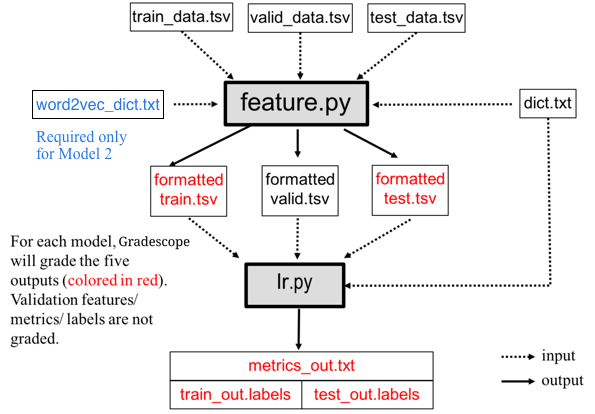
\includegraphics[width = 0.7\textwidth]{Pipeline_v2.png}
        \caption{Programming pipeline for sentiment analyzer based on binary logistic regression}
        \label{pipeline}
\end{figure}


This first program is \texttt{feature.\{py|java|cpp\}}, that converts raw data (e.g., \lstinline{train_data.tsv}, \lstinline{valid_data.tsv}, and \lstinline{test_data.tsv}) into formatted training, validation and test data based on the vocabulary information in the dictionary file \lstinline{dict.txt}. For Model 2, the program also takes in an additional feature dictionary file \lstinline{word2vec.txt}. To be specific, this program is to transfer the whole movie review text into a feature vector using some feature extraction methods. You should \emph{not} be folding in a bias term into the formatted output.
The formatted datasets should be stored in .tsv format. Details of formatted datasets will be introduced in Section~\ref{feature} and Section~\ref{format_output}.

The second program is \texttt{lr.\{py|java|cpp\}}, that implements a sentiment polarity analyzer using binary logistic regression. The file should learn the parameters of a binary logistic regression model that predicts a sentiment polarity (i.e. label) for the corresponding feature vector of each movie review. This program can either be implemented by folding in the bias term and weight or not. The program should output the labels of the training and test examples and calculate training and test error (percentage of incorrectly labeled reviews). 

\subsubsection{Feature Engineering} \label{feature}

Your implementation of \texttt{feature.\{py|java|cpp\}} should have an input argument \texttt{<feature\_flag>} that specifies one of two types of feature extraction structures that should be used by the logistic regression model. The two structures are illustrated below as probabilities of the labels given the inputs.

\subsubsection{Model 1}

Model 1 is written as $p\left(y^{(i)} \mid \boldsymbol{\phi}_1\left(\xv^{(i)}\right), \thetav\right)$. This model uses a \emph{bag-of-words} feature vector $\boldsymbol{\phi}_1\left(\xv^{(i)}\right) = \bf{1}_{occur}( \xv^{(i)},$ $\bf{Vocab})$ indicating which words in vocabulary $\bf{Vocab}$ of the dictionary occur at least once in the movie review example $\xv^{(i)}$. Specifically, there are $V=|\bf{Vocab}|$ entries in this indicator vector, and the $j$-th entry will be set to 1 if the $j$-th word in $\bf{Vocab}$ occurs at least once in the movie review. The $j$-th entry will be set to 0 otherwise. This bag-of-words model should be used when \texttt{<feature\_flag>} is set to 1.
    
\subsubsection{Model 2}

Model 2 is written as $p\left(y^{(i)} \mid \boldsymbol{\phi}_2\left(\xv^{(i)}\right), \thetav\right)$. This model makes use of \emph{word2vec} embeddings, which are reduced dimension  vector representations (features) of words. These feature vectors will be provided in \texttt{word2vec.txt}, which contains the \emph{word2vec} embeddings of \texttt{15k} words. Note that not every word in the movie review examples will be included in the provided \texttt{word2vec.txt} file.
    
For this model, there will be two steps in the feature engineering process: 
    
\begin{enumerate}
    \item First, we would like to exclude words from the review that are not included in the word2vec dictionary. Let ${I_i}$ be the set of indices of words in $\xv^{(i)}$ that are included in the \emph{word2vec} dictionary. Then, we can define $\xv\_\text{trim}^{(i)} = \xv^{(i)}[I_i]$, where $\xv^{(i)}[I_i]$ trims vector $\xv^{(i)}$ by only including elements of $\xv^{(i)}$ with indices in $I_i$. 
    \item Second, we want to take the trimmed vector $\xv\_\text{trim}^{(i)}$ and convert it to the final feature vector given by the following equation:
    $$\boldsymbol{\phi}_2\left(\xv^{(i)}\right) = \frac{1}{J} \sum_{j=1}^J word2vec(\xv\_\text{trim}^{(i)}_j) $$
    where $J$ denotes the number of words in $\xv\_\text{trim}^{(i)}$ and $\xv\_\text{trim}^{(i)}_j$ is the j-th word in $\xv\_\text{trim}^{(i)}$.
    
     In the given equation, $word2vec(\xv\_\text{trim}^{(i)}_j) \in \mathbb{R}^{300}$ is the \emph{word2vec} feature vector for the word $\xv\_\text{trim}^{(i)}_j$.
\end{enumerate}
    
The following \textbf{example} provides a reference for Model 2:

\begin{itemize}
    \item Let $\xv^{(i)}$ denote the sentence ``\texttt{a hot dog is not a sandwich because it is not\\ square}''.
    \item A toy \emph{word2vec} dictionary is given as follows (note that unlike the following text, contents in the actual input file given will be tab-separated): 
    \begin{lstlisting}
hot         0.1    0.2    0.3
not        -0.1    0.2   -0.3
sandwich    0.0   -0.2    0.4
square      0.2   -0.1    0.5
    \end{lstlisting}
    \item Then, $\xv\_\text{trim}^{(i)}$ denotes the trimmed review ``\texttt{hot not sandwich not square}''. Note that in this trimmed text, the words that are not in the \emph{word2vec} dictionary are excluded. Also note that we keep the order of words and do not de-duplicate words in the trimmed text.
    \item The feature for $\xv^{(i)}$ can be calculated as
        \begin{align*} \boldsymbol{\phi}_2(\xv^{(i)}) &= \frac{1}{5}\big( word2vec(\text{hot}) + 2 \cdot word2vec(\text{not}) + word2vec(\text{sandwich}) + word2vec(\text{square}) \big) \\
        &= \begin{bmatrix} 0.02 & 0.06 & 0.12 \end{bmatrix}^T.
        \end{align*}
\end{itemize}


The motivation of Model 2 is that pre-trained feature representations such as word2vec embeddings may provide richer information about sentiment of a sentence than the simpler bag-of-words features. You will observe whether using pre-trained word embeddings to build feature vectors will improve performance and accuracy.


\subsubsection{Command Line Arguments}
The autograder runs and evaluates the output from the files generated, using the following command (note \lstinline{feature} will be run before \lstinline{lr}):

\begin{tabbing}
For Python: \=\texttt{\$ \textbf{python} feature.\textbf{py} [args1\dots]}\\
\>\texttt{\$ \textbf{python} lr.\textbf{py} [args2\dots]}\\
For Java: \>\texttt{\$ \textbf{java} feature.\textbf{java} [args1\dots]}\\
\>\texttt{\$ \textbf{java} lr.\textbf{java} [args2\dots]}\\
For C++: \>\texttt{\$ \textbf{g++} feature.\textbf{cpp} ./a.out [args1\dots]}\\
\>\texttt{\$ \textbf{g++} lr.\textbf{cpp} ./a.out [args2\dots]}
\end{tabbing}

Where above \texttt{[args1\dots]} is a placeholder for nine command-line arguments: \texttt{<train\_input>}\newline \texttt{<validation\_input> <test\_input> <dict\_input> <formatted\_train\_out> \newline <formatted\_validation\_out>  <formatted\_test\_out> <feature\_flag> \newline <feature\_dictionary\_input>}. These arguments are described in detail below:
\begin{enumerate}
    \item \texttt{<train\_input>}: path to the training input \texttt{.tsv} file (see Section~\ref{dataset})
    \item \texttt{<validation\_input>}: path to the validation input \texttt{.tsv} file (see Section~\ref{dataset})
    \item \texttt{<test\_input>}: path to the test input \texttt{.tsv} file (see Section~\ref{dataset})
    \item \texttt{<dict\_input>}: path to the dictionary input \texttt{.txt} file (see Section~\ref{dataset})
    \item \texttt{<formatted\_train\_out>}: path to output \texttt{.tsv} file to which the feature extractions on the \emph{training} data should be written (see Section~\ref{format_output})
    \item \texttt{<formatted\_validation\_out>}: path to output \texttt{.tsv} file to which the feature extractions on the \emph{validation} data should be written (see Section~\ref{format_output})
    \item \texttt{<formatted\_test\_out>}: path to output \texttt{.tsv} file to which the feature extractions on the \emph{test} data should be written (see Section~\ref{format_output})
    \item \texttt{<feature\_flag>}: integer taking value 1 or 2 that specifies whether to construct the Model 1 feature set or the Model 2 feature set (see Section~\ref{feature})---that is, if \lstinline{feature_flag}==1 use Model 1 features; if \lstinline{feature_flag}==2 use Model 2 features
    \item \texttt{<feature\_dictionary\_input>}: path to the word2vec feature dictionary \texttt{.tsv} file (see Section~\ref{dataset}). 
\end{enumerate}


Likewise, \texttt{[args2\dots]} is a placeholder for eight command-line arguments: \texttt{<formatted\_train\_input>}\newline \texttt{<formatted\_validation\_input> <formatted\_test\_input> <dict\_input> <train\_out> \newline <test\_out> <metrics\_out> <num\_epoch>}. These arguments are described in detail below:
\begin{enumerate}
    \item \texttt{<formatted\_train\_input>}: path to the formatted training input \texttt{.tsv} file (see Section~\ref{format_output})
    \item \texttt{<formatted\_validation\_input>}: path to the formatted validation input \texttt{.tsv} file (see Section~\ref{format_output})
    \item \texttt{<formatted\_test\_input>}: path to the formatted test input \texttt{.tsv} file (see Section~\ref{format_output})
    \item \texttt{<dict\_input>}: path to the dictionary input \texttt{.txt} file (see Section~\ref{dataset})
    \item \texttt{<train\_out>}: path to output \texttt{.labels} file to which the prediction on the \emph{training} data should be written (see Section~\ref{output})
    \item \texttt{<test\_out>}: path to output \texttt{.labels} file to which the prediction on the \emph{test} data should be written (see Section~\ref{output})
    \item \texttt{<metrics\_out>}: path of the output \texttt{.txt} file to which metrics such as train and test error should be written (see Section~\ref{metrics})
    %\item \texttt{<model\_out>}: path of the output \texttt{.txt} file to which the model parameters should be written (see Section~\ref{model})
    \item \texttt{<num\_epoch>}: integer specifying the number of times SGD loops through all of the training data (e.g., if \texttt{<num\_epoch>} equals 5, then each training example will be used in SGD 5 times). 
\end{enumerate}

As an example, if you implemented your program in Python, the following two command lines would run your programs on the data provided in the handout for 500 epochs using the features from Model 1.

\begin{lstlisting}[language=Shell]
$ python feature.py largedata/train_data.tsv largedata/valid_data.tsv
largedata/test_data.tsv dict.txt largeoutput/formatted_train.tsv
largeoutput/formatted_valid.tsv largeoutput/formatted_test.tsv
1 word2vec.txt

$ python lr.py largeoutput/formatted_train.tsv 
largeoutput/formatted_valid.tsv largeoutput/formatted_test.tsv 
dict.txt largeoutput/train_out.labels largeoutput/test_out.labels 
largeoutput/metrics_out.txt 500

\end{lstlisting}

\begin{notebox}
{\bf Important Note:} You will not be writing out the predictions on validation data, only on train and test data. The validation data is \emph{only} used to give you an estimate of held-out negative log-likelihood at the end of each epoch during training. You are asked to graph the negative log-likelihood vs. epoch of the validation and training data in Programming Empirical Questions section. \footnote{For this assignment, we will always specify the number of epochs. However, a more mature implementation would monitor the performance on validation data at the end of each epoch and stop SGD when this validation log-likelihood appears to have converged. You should \textbf{\emph{not}} implement such a convergence check for this assignment.} 
\end{notebox}

\subsection{Program Outputs}

\subsubsection{Output: Formatted Data Files} \label{format_output}
Your \lstinline{feature} program should write three output \texttt{.tsv} files converting original data to formatted data on \texttt{<formatted\_train\_out>}, \texttt{<formatted\_valid\_out>}, and \texttt{<formatted\_test\_out>}. Each should contain the formatted presentation for each example printed on a new line. Use \lstinline{\n} to create a new line. The format for each line should exactly match label\lstinline{\t}value1\lstinline{\t}value2\lstinline{\t}value3\lstinline{\t}...valueM\lstinline{\n}

Where above, the first column is label, and the rest are "value" feature elements. Value is the value of the feature at index \texttt{i} of the formatted output row. In this assignment, for Model 1 the value is one or zero depending on whether dictionary word \texttt{i} is present in the sentence. For Model 2, the rows are the summed up word2vec vectors for all the words present in the dictionary. Columns are separated using a table character, \lstinline{\t}. The handout contains example \texttt{<formatted\_train\_out>}, \newline \texttt{<formatted\_valid\_out>}, and \texttt{<formatted\_test\_out>} for your reference.

The formatted output will be checked separately by the autograder by running your \lstinline{feature} program on some unseen datasets and evaluating your output file against the reference formatted files. For Model 2, please round to 6 decimal places (e.g. 0.123456). Examples of content of formatted output file are given below.

For Model 1:
\begin{lstlisting}
0	1	1	0	1	0	1	1	...
0	1	0	0	1	0	1	1	...
1	1	1	1	0	0	1	0	...
1	0	1	1	0	0	0	1	...
\end{lstlisting}
For Model 2:
\begin{lstlisting}
1.000000	-0.217109	-0.157321	-0.193579	...
0.098980	-1.059955	0.309624	-0.397892	...
0.560687	1.878663	-1.354379	0.148609	...
1.731375	-0.843260	1.445480	-2.125001	...
\end{lstlisting}



\subsubsection{Output: Labels Files} \label{output}
Your \lstinline{lr} program should produce two output \texttt{.labels} files containing the predictions of your model on training data (\texttt{<train\_out>}) and test data (\texttt{<test\_out>}). Each should contain the predicted labels for each example printed on a new line. Use \lstinline{\n} to create a new line. 

Your labels should exactly match those of a reference implementation -- this will be checked by the autograder by running your program and evaluating your output file against the reference solution. Examples of the content of the output file are given below.

\begin{lstlisting}
0
0
1
0
\end{lstlisting}

\subsubsection{Output Metrics} \label{metrics}
Generate a file where you report the following metrics: 

\begin{description}

\item[error] After the final epoch (i.e. when training has completed fully), report the final training error \newline \lstinline{error(train)} and test error \lstinline{error(test)}. 
\end{description}

All of your reported numbers should be within 0.01 of the reference solution and round the error values to 6 decimal places. The following is the reference solution for large dataset with Model 1 feature structure after 500 training epochs. See \newline \lstinline{model1_metrics_out.txt} in the handout.

 % 0.002857
 % 0.240000
\begin{lstlisting}
error(train): 0.049167
error(test): 0.150000
\end{lstlisting}

Take care that your output has the exact same format as shown above. Each line should be terminated by a Unix line ending \lstinline{\n}. There is a whitespace character after the colon.

\subsection{Evaluation and Submission}

\subsubsection{Evaluation}

Gradescope will test your implementations on hidden datasets with the same format as the two datasets provided in the handout. \lstinline{feature} program and \lstinline{lr} program will be tested separately. To ensure that your code can pass the gradescope tests in under 5 minutes (the maximum time length) be sure that your code can complete 500-epoch (for model 1 and 2, respectively) training and finish predictions through all of the data in the \lstinline{largedata} folder in around one minute.


\subsubsection{Requirements}
Your implementation must satisfy the following requirements:
\begin{itemize}
    \item The \texttt{feature.\{py|java|cpp\}} must produce a dense representation of the data according to the \texttt{feature\_flag}. We will use unseen data to test your feature output separately. (see Section~\ref{format_output} and Section~\ref{feature} on feature engineering for details on how to do this). 
    \item Ignore the words not in the vocabulary of \lstinline{dict.txt} when the analyzer encounters one in the test or validation data.
    \item Initialize all model parameters to $0$.
    \item Use stochastic gradient descent (SGD) to optimize the parameters for a binary logistic regression model. The number of times SGD loops through all of the training data (\texttt{num\_epoch}) will be specified as a command line flag. Set your learning rate as a constant $\alpha = 0.01$ for both Model 1 and Model 2 when comparing your outputs with the reference output provided in the handout (you will need to change the learning rate for some of the empirical questions, however).
    \item Perform stochastic gradient descent updates on the training data \textbf{in the order that the data is given in the input file}. Although you would typically shuffle training examples when using stochastic gradient descent, in order to autograde the assignment, we ask that you {\bf DO NOT} shuffle trials in this assignment.
    \item Be able to select which one of two feature extractions you will use in your logistic regression model using a command line flag (see Section~\ref{feature})
    \item Do not hard-code any aspects of the datasets into your code. We will autograde your programs on multiple (hidden) datasets that include different attributes and output labels.
\end{itemize}

\subsubsection{Hints}
Careful planning will help you to correctly and concisely implement your program. Here are a few \emph{hints} to get you started.
\begin{itemize}
    \item Work through the written component.
    \item (\textbf{Python only}) We strongly recommend you to write your own text parser rather than using parser provided in various packages.
    \item For reading in the word2vec embeddings, and to read the formatted inputs, we strongly recommend you utilize a linear algebra library to speed up vector computations.
    \item Be sure to check that the output from your \texttt{feature.\{py|java|cpp\}} matches the reference output given exactly before proceeding to \texttt{lr.\{py|java|cpp\}}.
    \item Write a function that takes a single SGD step on the $i$-th training example. Such a function should take as input the model parameters, the learning rate, and the features and label for the $i$-th training example. It should update the model parameters in place by taking one stochastic gradient step.
    \item Write a function that takes in a set of features, labels, and model parameters and then outputs the error (percentage of labels incorrectly predicted). You can also write a separate function that takes the same inputs and outputs the negative log-likelihood of the regression model.
    \item You can either treat the bias term as separate variable, or fold it into the parameter vector. In either case, make sure you update the bias term correctly.  
\end{itemize}

\subsubsection{Gradescope Submission}

You should submit your \texttt{feature.\{py|java|cpp\}} and %\newline 
\texttt{lr.\{py|java|cpp\}} to Gradescope.
Note: please do not use other file names. This will cause problems for the autograder to correctly detect and run your code.

    
    
%%%%%%%%%%%%%%%%%%%%%%%%%%%%%%%%%%%%%%%%%%%%%%%%%%%%%%%%%%%%%%%%%%%%%%%%%%%%%%%%%%%



\newpage

\appendix
% TODO: Discussion of sparse gradient update
% TODO: Numerically stable softmax


\section{Implementation Details for Logistic Regression}

\subsection{Examples of Features}

Here we provide examples of the features constructed by Model 1 and Model 2. Table \ref{tab:inputfile} shows an example input file, where column $i$  indexes the $i$-th movie review example. Rather than working directly with this input file, you should transform the sentiment/text representation into a label/feature vector representation.

Table \ref{tab:model1dense} shows the dense occurrence-indicator representation expected for Model 1. The size of each feature vector (i.e. number of feature columns in the table) is equal to the size of the entire vocabulary of words stored in the given \lstinline{dict.txt} (this dictionary is actually constructed from the same training data in \lstinline{largeset}). Each row corresponds to a single example, which we have indexed by $i$.










\begin{table}[p]
    \centering
%
\begin{tabular}{cll}
\toprule
{\bf example index} $i$  & {\bf sentiment $y^{(i)}$ } & {\bf review text $\xv^{(i)}$ }\\
\midrule
1 & pos & apple boy , cat dog \\
2 & pos & boy boy : dog dog ; dog dog . dog egg egg \\
3 & neg & apple apple apple apple boy cat cat dog \\
4 & neg & egg fish \\

\bottomrule
\end{tabular}
%
    \caption{Abstract representation of the input file format.  The $i$th row of this file will be used to construct the $i$th training example using either Model 1 features or Model 2 features.}
    \label{tab:inputfile}
\end{table}


\begin{table}[p]
    \centering
%
\begin{tabular}{clllllllllllll}
\toprule
$i$ & {\bf label} $y^{(i)}$ & \multicolumn{12}{l}{ {\bf features} $\xv^{(i)}$  }\\
& & \rot{\tt zoo} & \rot{$\ldots$} & \rot{\tt apple} & \rot{\tt boy} & \rot{\tt cat} & \rot{\tt dog} & \rot{\tt egg} & \rot{\tt fish} & \rot{\tt girl} & \rot{\tt head} & \rot{$\ldots$} & \rot{\tt zero} \\
\midrule
1 & 1                    & 0 & $\ldots$ & 1 & 1 & 1 & 1 & 0 & 0 & 0 & 0 & $\ldots$ & 0 \\ 
2 & 1                    & 0 & $\ldots$ & 0 & 1 & 0 & 1 & 1 & 0 & 0 & 0 & $\ldots$ & 0 \\ 
3 & 0                    & 0 & $\ldots$ & 1 & 1 & 1 & 1 & 0 & 0 & 0 & 0 & $\ldots$ & 0 \\ 
4 & 0                    & 0 & $\ldots$ & 0 & 0 & 0 & 0 & 1 & 1 & 0 & 0 & $\ldots$ & 0 \\ 

\bottomrule
\end{tabular}
%
    \caption{Dense feature representation for Model 1 corresponding to the input file in Table \ref{tab:inputfile}. The $i$th row corresponds to the $i$th training example. Each dense feature has the size of the vocabulary in the dictionary. Punctuations are excluded.}
    \label{tab:model1dense}
\end{table}


\subsection{Efficient Computation of the Dot-Product} \label{efficientdp}

Using a for loop to perform a dot product is very slow and inefficient, especially in python. There are linear algebra libraries optimized to compute the dot product for you. With that said, you may find the following linear algebra libraries for efficient dot product computation useful:

NumPy (Python)

\begin{lstlisting}[language=Python]
np.dot(A, B)
\end{lstlisting}


EJML (Java)
\begin{lstlisting}[language=Java]
dot(A, B)
\end{lstlisting}

ND4J (Java)
\begin{lstlisting}[language=Java]
dot(A, B)
\end{lstlisting}

Eigen (C++)
\begin{lstlisting}[language=C++]
A.dot(B)
\end{lstlisting}

where $A$ and $B$ are vectors or matrices
\end{document}